\section{Interpolazione Polinomiale} 

\begin{exercise}[4.1] 
Trovare un polinomio $p(x)$ che interpola la funzione $f(x) = 4x^{2} -12x +1$
nei punti di ascissa $x_{i} = i$, con $ i \in \{ 0,\ldots, 4 \}$.
\end{exercise}
Per l'implementazione vedere il codice \nameref{subsec:exercise41} e per la 
sua esecuzione lanciare lo script \nameref{subsec:scriptForExercise41}.
\begin{center} 
% GNUPLOT: LaTeX picture with Postscript
\begingroup
  \makeatletter
  \providecommand\color[2][]{%
    \GenericError{(gnuplot) \space\space\space\@spaces}{%
      Package color not loaded in conjunction with
      terminal option `colourtext'%
    }{See the gnuplot documentation for explanation.%
    }{Either use 'blacktext' in gnuplot or load the package
      color.sty in LaTeX.}%
    \renewcommand\color[2][]{}%
  }%
  \providecommand\includegraphics[2][]{%
    \GenericError{(gnuplot) \space\space\space\@spaces}{%
      Package graphicx or graphics not loaded%
    }{See the gnuplot documentation for explanation.%
    }{The gnuplot epslatex terminal needs graphicx.sty or graphics.sty.}%
    \renewcommand\includegraphics[2][]{}%
  }%
  \providecommand\rotatebox[2]{#2}%
  \@ifundefined{ifGPcolor}{%
    \newif\ifGPcolor
    \GPcolortrue
  }{}%
  \@ifundefined{ifGPblacktext}{%
    \newif\ifGPblacktext
    \GPblacktexttrue
  }{}%
  % define a \g@addto@macro without @ in the name:
  \let\gplgaddtomacro\g@addto@macro
  % define empty templates for all commands taking text:
  \gdef\gplbacktext{}%
  \gdef\gplfronttext{}%
  \makeatother
  \ifGPblacktext
    % no textcolor at all
    \def\colorrgb#1{}%
    \def\colorgray#1{}%
  \else
    % gray or color?
    \ifGPcolor
      \def\colorrgb#1{\color[rgb]{#1}}%
      \def\colorgray#1{\color[gray]{#1}}%
      \expandafter\def\csname LTw\endcsname{\color{white}}%
      \expandafter\def\csname LTb\endcsname{\color{black}}%
      \expandafter\def\csname LTa\endcsname{\color{black}}%
      \expandafter\def\csname LT0\endcsname{\color[rgb]{1,0,0}}%
      \expandafter\def\csname LT1\endcsname{\color[rgb]{0,1,0}}%
      \expandafter\def\csname LT2\endcsname{\color[rgb]{0,0,1}}%
      \expandafter\def\csname LT3\endcsname{\color[rgb]{1,0,1}}%
      \expandafter\def\csname LT4\endcsname{\color[rgb]{0,1,1}}%
      \expandafter\def\csname LT5\endcsname{\color[rgb]{1,1,0}}%
      \expandafter\def\csname LT6\endcsname{\color[rgb]{0,0,0}}%
      \expandafter\def\csname LT7\endcsname{\color[rgb]{1,0.3,0}}%
      \expandafter\def\csname LT8\endcsname{\color[rgb]{0.5,0.5,0.5}}%
    \else
      % gray
      \def\colorrgb#1{\color{black}}%
      \def\colorgray#1{\color[gray]{#1}}%
      \expandafter\def\csname LTw\endcsname{\color{white}}%
      \expandafter\def\csname LTb\endcsname{\color{black}}%
      \expandafter\def\csname LTa\endcsname{\color{black}}%
      \expandafter\def\csname LT0\endcsname{\color{black}}%
      \expandafter\def\csname LT1\endcsname{\color{black}}%
      \expandafter\def\csname LT2\endcsname{\color{black}}%
      \expandafter\def\csname LT3\endcsname{\color{black}}%
      \expandafter\def\csname LT4\endcsname{\color{black}}%
      \expandafter\def\csname LT5\endcsname{\color{black}}%
      \expandafter\def\csname LT6\endcsname{\color{black}}%
      \expandafter\def\csname LT7\endcsname{\color{black}}%
      \expandafter\def\csname LT8\endcsname{\color{black}}%
    \fi
  \fi
  \setlength{\unitlength}{0.0500bp}%
  \begin{picture}(7680.00,5760.00)%
    \gplgaddtomacro\gplbacktext{%
      \colorrgb{0.00,0.00,0.00}%
      \put(866,634){\makebox(0,0)[r]{\strut{}-500}}%
      \colorrgb{0.00,0.00,0.00}%
      \put(866,1573){\makebox(0,0)[r]{\strut{}0}}%
      \colorrgb{0.00,0.00,0.00}%
      \put(866,2511){\makebox(0,0)[r]{\strut{}500}}%
      \colorrgb{0.00,0.00,0.00}%
      \put(866,3450){\makebox(0,0)[r]{\strut{}1000}}%
      \colorrgb{0.00,0.00,0.00}%
      \put(866,4388){\makebox(0,0)[r]{\strut{}1500}}%
      \colorrgb{0.00,0.00,0.00}%
      \put(866,5327){\makebox(0,0)[r]{\strut{}2000}}%
      \colorrgb{0.00,0.00,0.00}%
      \put(998,414){\makebox(0,0){\strut{}-20}}%
      \colorrgb{0.00,0.00,0.00}%
      \put(1742,414){\makebox(0,0){\strut{}-15}}%
      \colorrgb{0.00,0.00,0.00}%
      \put(2486,414){\makebox(0,0){\strut{}-10}}%
      \colorrgb{0.00,0.00,0.00}%
      \put(3230,414){\makebox(0,0){\strut{}-5}}%
      \colorrgb{0.00,0.00,0.00}%
      \put(3974,414){\makebox(0,0){\strut{}0}}%
      \colorrgb{0.00,0.00,0.00}%
      \put(4718,414){\makebox(0,0){\strut{}5}}%
      \colorrgb{0.00,0.00,0.00}%
      \put(5462,414){\makebox(0,0){\strut{}10}}%
      \colorrgb{0.00,0.00,0.00}%
      \put(6206,414){\makebox(0,0){\strut{}15}}%
      \colorrgb{0.00,0.00,0.00}%
      \put(6950,414){\makebox(0,0){\strut{}20}}%
    }%
    \gplgaddtomacro\gplfronttext{%
    }%
    \gplbacktext
    \put(0,0){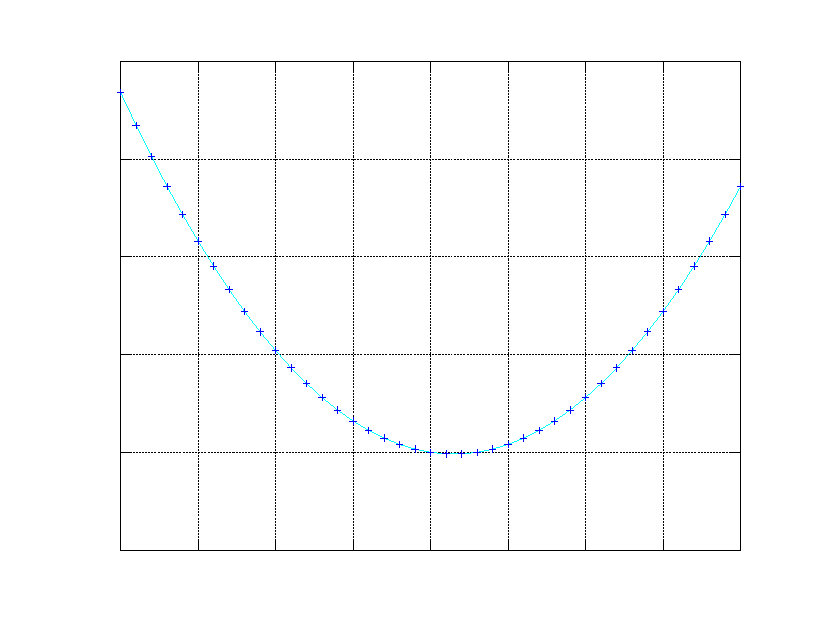
\includegraphics{ApprossimazioneFunzioni/exercise41PlotOutput}}%
    \gplfronttext
  \end{picture}%
\endgroup

\end{center}
In cyan \`e reppresentata la curva della funzione $f$, mentre con i simboli
$+$ sono rappresentati i punti interpolati dal polinomio $p$.

\begin{exercise}[4.2] 
Per il testo dell'esercizio consulare il libro di testo.
\end{exercise}
\begin{proof}
L'algoritmo riportato implementa questo schema (utilizzo gli indici nella
notazione usata nella formulazione matematica, quindi sono zero-based):
\begin{displaymath}
\begin{split}
	p^{(0)}(x) &= a_{n} \\
	p^{(i+1)}(x) &= p^{(i)}x + a_{n-i} 
\end{split}
\end{displaymath}
con $p^{(i)}$ indico il valore di $p$ all'$i$-esimo passo dei esecuzione. 
Se considero il valore di $p$ ad un generico passo $i$ di esecuzione si
osserva che ha questa struttura:
\begin{displaymath}
\begin{split}
	p^{(i)}(x) &= (a_{n}x^{i-1} + a_{n-1}x^{i-2} + \ldots + a_{n-i+1})x + a_{n-i}\\
	&= a_{n}x^{i} + a_{n-1}x^{i-1} + \ldots + a_{n-i+1}x + a_{n-i}
\end{split}
\end{displaymath}
Il polinomio $p^{(i)}$ \`e di grado $i$, quindi saturando l'indice $i$ arrivando
a calcolare $p^{n}$, si ottiene il polinomio:
\begin{displaymath}
	p(x) = p^{(n)}(x) = a_{n}x^{n} + a_{n-1}x^{n-1} + \ldots + a_{1}x + a_{0}
\end{displaymath}
Ovvero quello che si chiede nel problema.
\end{proof}

\begin{exercise}[4.3] 
Per il testo dell'esercizio consulare il libro di testo.
\end{exercise}
\begin{proof}
Dimostro i punti del \emph{Lemma 4.1}:
\begin{enumerate}
  \item \label{exercise43proofPoint1} questa \`e la forma di un generico
  polinomio $k$ della base di Lagrange di grado $n$:
  \begin{displaymath}
  L_{kn}(x) = \frac{(x-x_{0}) \cdots (x-x_{k-1})(x-x_{k+1})\cdots (x-x_{n})}
  	{(x_{k}-x_{0}) \cdots (x_{k}-x_{k-1})(x_{k}-x_{k+1})\cdots (x_{k}-x_{n})}
  \end{displaymath}
  Se valuto il polinomio $L_{kn}(x_{i})$ in una generica ascissa di
  interpolazione $x_{i}$ posso avere due casi:
  \begin{itemize}
    \item se $i \not = k$, allora $x_{i} \in \{
    x_{0},\ldots,x_{k-1},x_{k+1},\ldots,x_{n} \}$ ma questo fa si che uno dei
    fattori del numeratore abbia la forma $(x_{i} - x_{i}) = 0$ che annulla la
    produttoria:
    \begin{displaymath}
  L_{kn}(x_{i\not = k}) = \frac{(x_{i}-x_{0}) \cdots
  (x_{i}-x_{k-1})(x_{i}-x_{k+1})\cdots (x_{i}-x_{i}) \cdots (x_{i}-x_{n})}
  	{(x_{k}-x_{0}) \cdots (x_{k}-x_{k-1})(x_{k}-x_{k+1})\cdots (x_{k}-x_{n})} = 0
  \end{displaymath}
  Osservazione: ho inserito il termine che si annulla pi\`u a destra, ma il
  posizionamento \`e da ritenersi non influente in quanto per il prodotto
  l'ordine dei fattori non influisce ed inoltre \`e dipendente da $i$.
    \item se $i = k$ allora ottengo
    \begin{displaymath}
  L_{kn}(x_{i = k}) = \frac{(x_{k}-x_{0}) \cdots
  (x_{k}-x_{k-1})(x_{k}-x_{k+1})\cdots (x_{k}-x_{n})}
  	{(x_{k}-x_{0}) \cdots (x_{k}-x_{k-1})(x_{k}-x_{k+1})\cdots (x_{k}-x_{n})} = 1
  \end{displaymath}
  \end{itemize}
  
  \item i polinomi della base di Lagrange hanno grado esatto $n$ in quanto per
  definizione del generico polinomio $k$ si ha:
  \begin{displaymath}
  	L_{kn}(x) = \prod_{j=0 \quad j \not = k}^{n}{\frac{x-x_{j}}{x_{k}-x_{j}}}
  \end{displaymath}
  l'indice della produttoria ``corre'' da $0$ a $n$, indicizzando $n+1$
  posizioni, ma la $k$-esima posizione viene saltata, quindi vengono eseguiti
  $n$ prodotti, di conseguenza il termine di grado massimo \`e $x^{n}$.
  Inoltre posso dividera la produttoria in questo modo:
  \begin{displaymath}
  	L_{kn}(x) = \frac{\prod_{j=0; j \not =
  	k}^{n}{x-x_{j}}}{\prod_{j=0; j \not =
  	k}^{n}{x_{k}-x_{j}}}
  \end{displaymath}
  la quantit\`a al denominatore non dipende dall'ascissa $x$ in input, quindi si
  pu\`o sviluppare il prodotto al numeratore, ottenendo un polinomio di grado
  $n$, con coefficiente uguale a $1$, poi moltiplicare per la costante al
  denominatore, ottenendo il termine di grado massimo:
  \begin{displaymath}
  	a_{n}x^{n} = \frac{1}{\prod_{j=0; j \not = k}^{n}{x_{k}-x_{j}}} x^{n}
  \end{displaymath}
  
  \item per dimostrare che i polinomi $L_{kn}(x)$ formano una base per  
  $\prod_{n}$ allora devo dimostrare:
  \begin{displaymath}
  	\alpha_{0}L_{0n}(x)+ \ldots + \alpha_{n}L_{nn}(x) = 0 \Leftrightarrow
  	\alpha_{0} = \ldots = \alpha_{n} = 0 
  \end{displaymath}
  Il verso $\Leftarrow$ \`e ovvio. Per il verso $\Rightarrow$ invece valuto
  la combinazione lineare dei polinomi in una generica ascissa di
  interpolazione $x_{i}$ ottenendo:
  \begin{displaymath}
  	\alpha_{0}L_{0n}(x_{i})+ \ldots + \alpha_{n}L_{nn}(x_{i}) = 0  
  \end{displaymath}
  Per il punto \ref{exercise43proofPoint1} i termini $\alpha_{k}L_{kn}(x_{i}) =
  0$ se $i \not = k$, quindi rimane il solo elemento $\alpha_{i}L_{in}(x_{i})$. 
  Ma, sempre per il punto \ref{exercise43proofPoint1} vale $L_{in}(x_{i}) = 1$,
  quindi:
  \begin{displaymath}
  	0 = \alpha_{i}L_{in}(x_{i}) = \alpha_{i}  
  \end{displaymath}
  Ripetendo questo ragionamento per ogni ascissa di interpolazione si ottiene
  $\alpha_{0} = \ldots = \alpha_{n} = 0$ e il verso risulta dimostrato.
\end{enumerate}
\end{proof}

\begin{exercise}[4.4] 
Per il testo dell'esercizio consulare il libro di testo.
\end{exercise}
\begin{proof}
Dimostro i punti del \emph{Lemma 4.2}:
\begin{enumerate}
  \item	\label{exercise44ProofPoint1} 
  $w_{k+1}(x) = (x - x_{k})w_{k}(x) = (x - x_{k})(x - x_{k-1})w_{k-1}(x)
   = \ldots = (x - x_{k})\cdots (x - x_{0}) = \prod_{j = 0}^{k}{(x - x_{j})}$
   \item come si vede dal punto
   \ref{exercise44ProofPoint1}, valutare $w_{k}(x)$ richiede eseguire $k$
   prodotti, per cui si ottiene un polinomio di grado $k$, quindi $w_{k}(x) \in
   \prod_{k}$
   \item valutare il polinomio $w_{k}$ in una delle ascisse di interpolazione
   $x_{i}$ con $i<k$, ovvero $w_{k}(x_{i})$ si ha che uno dei fattori di
   $w_{k}(x_{i}) = (x_{i} - x_{k-1})\cdots (x_{i} - x_{i}) \cdots (x_{i} -
   x_{0})$ si annulli, annullando di conseguenza tutta la somma, quindi vale
   $i<k \Rightarrow w_{k}(x_{i}) = 0 $.
   \item per dimostrare che i polinomi $w_{k}(x)$ formano una base per  
  $\prod_{k}$ allora devo dimostrare:
  \begin{displaymath}
  	\alpha_{0}w_{0}(x)+ \ldots + \alpha_{k}w_{k}(x) = 0 \Leftrightarrow
  	\alpha_{0} = \ldots = \alpha_{k} = 0 
  \end{displaymath}
  Sviluppo per chiarezza la precedente combinazione lineare:
  \begin{displaymath}
  	\alpha_{0} + \alpha_{1}(x - x_{0}) + \alpha_{2}(x - x_{1})(x - x_{0}) \ldots
  	+ \alpha_{k}(x - x_{k-1})\cdots(x - x_{0}) = 0
  \end{displaymath}
  Il verso $\Leftarrow$ \`e ovvio. Per il verso $\Rightarrow$ invece valuto
  la combinazione lineare dei polinomi in una generica ascissa di
  interpolazione $x_{i} \in \{ x_{0}, \ldots, x_{k} \}$ ottenendo:
  \begin{displaymath}
  	\alpha_{0}w_{0}(x_{i})+ \ldots + \alpha_{k}w_{k}(x_{i}) = 0   
  \end{displaymath}
  Posso ragionare distinguendo due casi:
  \begin{itemize}
    \item se $i = k$ allora $\forall j \in \{ 0, k \}:w_{j}(x_{i}) \not = 0$, in
    quanto per ipotesi le ascisse di interpolazione sono distinte due a due.
    Per ipotesi di questo verso, la combinazione lineare degli elementi della
    base deve annullarsi, quindi affinche l'ipotesi venga rispettata deve valere 
    $\alpha_{0} = \ldots = \alpha_{k} = 0$
    \item se $i < k$ allora tutti i termini della forma $w_{j}(x_{i}) = 0$ se
    $i < j$. Possono per\`o rimanere dei termini (verso le prime posizioni
    della produttoria) per cui $w_{r}(x_{i}) \not = 0$ se
    $i \geq r$. Ma per questi termini posso ragionare come fatto nel caso di $i
    < k$, ottenendo che $\alpha_{0} = \ldots = \alpha_{r} = 0$.
  \end{itemize}
   Ripetendo questo ragionamento per ogni ascissa di interpolazione si ottiene
  $\alpha_{0} = \ldots = \alpha_{k} = 0$ e il verso risulta dimostrato.
 \end{enumerate}
\end{proof}